% TeX root = ../../paper.tex
%
\section{Implementation}\label{sec:implementation}


The base of the \emph{Petrinets Testing} language is the MontiCore Language Workbench~\cite{rumpe2017monticore} 6.1.0 which is a fully featured framework for the development of domain-specific languages. Based on the grammar that we present above, it is able to generate, among many other tools, a parser for models that conform to the grammar which also translates the model to a powerful and easy to manipulate data structure, the Abstract Syntax Tree (AST).
As code is generated even before compile time it also provides a development infrastructure that is specifically suited to work with our DSL and is easy to extend with more features, including code generation.
This also means that only the parts that specifically concern the functionality of the language models had to be implemented.

We use unit testing to evaluate our implementation, aiming for a high degree of test coverage.


\begin{figure}
  \centering
  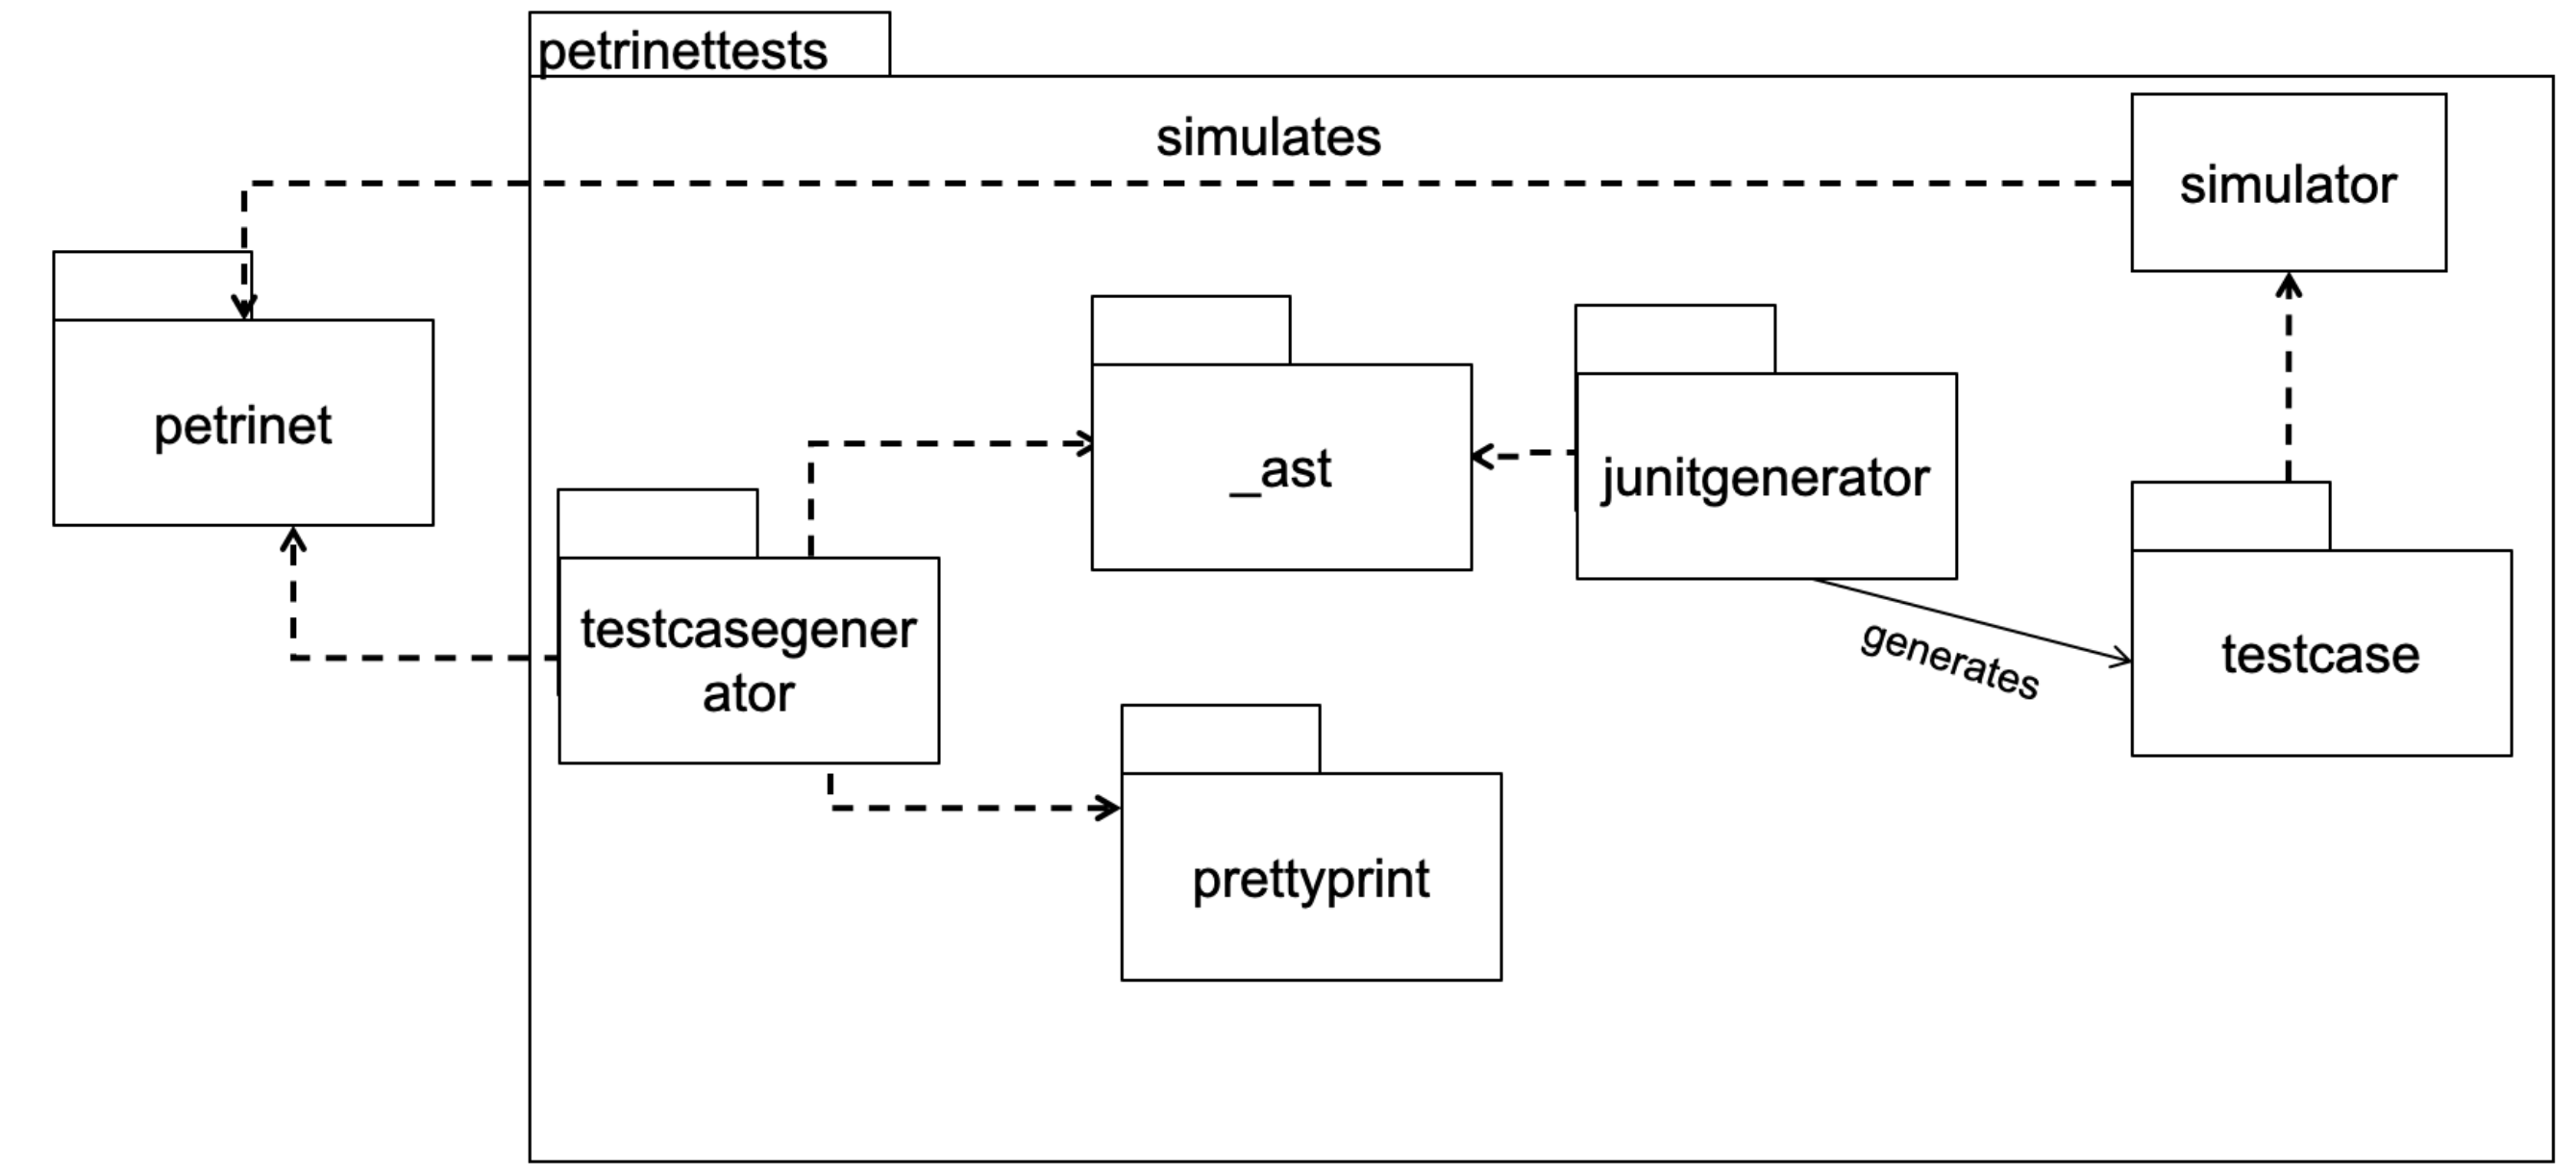
\includegraphics[width=\textwidth]{src/pic/architecture.png}
  \caption{The \emph{Petrinets Testing} language Architecture}
  \label{fig:architecture}
\end{figure}


Figure \ref{fig:architecture} shows the top-level architecture based on packages as well as their interactions. \textbf{petrinet} here stands for the \emph{petrinet4analysis} language. In the following, we describe the main roles of the individual packages.


\begin{itemize}
	\item \textbf{testcasegenerator} contains the classes that implement the automatic generation of test cases based on models provided as \emph{petrinet4analysis} AST. The mechanism that is implemented here is explained in detail in \ref{sec:generation}.
	\item \textbf{prettyprint} Using the PrettyPrinter, it is possible to inspect a \emph{Petrinet Testing} model by printing it to a string. It makes use of the IndentPrinter provided by MontiCore, as well as the Visitor pattern. Its main use case is the export of ASTs that have been generated by the \textbf{testcasegenerator} package.
	\item \textbf{junitgenerator} provides functionality of generating executable testcases from \textit{Petrinet Testing} models. This makes use of the MontiCore support for generation. Several templates are defined in the \textit{FreeMarker} template language and passed to MontiCore along with the AST to generate from. This results in Java code that implements a JUnit test case.
	\item \textbf{simulator} could be seen as a run-time environment for generated test cases. The generated test cases require on this package which is able to perform operations on \emph{petrinet4analysis} ASTs needed to perform the individual test steps. This includes setting a marking on a petri net and updating the marking based on transitions.
\end{itemize}

\subsubsection{Tool} In additon to that, we provide a command line interface as a user interface to our toolset. It supports both the generation of \textit{Petrinet Testing} models from \textit{petrinet4analysis} models using the \textbf{testcasegenerator} package, as well as the generation of JUnit tests from \textit{Petrinet Testing} models. The tool is accessible through the command \texttt{java -jar petrinet-tests.jar}, where the file petrinet-tests.jar has to be the fully assembled jar file. The \texttt{--help} flag provides user information about the tool.

\subsubsection{Running tests}
We provide a separate maven module \textit{petrinet-tests-runner} that is able to parse models and execute all defined tests automatically. Both \textit{petrinet4analysis} and \textit{Petrinet Testing} models can be placed in to the module's \texttt{src/main/resources} directory to be considered. The generated files will be stored in the directory \texttt{target/generated-test-sources}.

This process is already included in the standard maven build process and can therefore be triggered by running \texttt{mvn install}.

\subsubsection{Workflow}
A workflow that combines several use cases of our toolset could therefore look as follows.
First, the user defines the model they wish to test as a \emph{petrinet4analysis} model. Along with that, they can define hand-written test cases and write them using \textit{Petrinet Testing} models.
Then, using the PetrinetTestsTool, they can trigger the automatic generation of testcases described in section \ref{sec:generation}. This will generate additional \textit{Petrinet Testing} model files. 
Both the \textit{petrinet4analyis} and the \textit{Petrinet Testing} models can be placed into the folder mentioned above. By running the maven goal install, the run of the runner module described above is triggered. It reads all defined models and generates executable JUnit tests that execute the defined test cases. As the tests are directly run, the user is able to read the test results directly from the console.

\subsection{Adaptations to \emph{petrinet4analysis}}

In order to be compatible with \textit{petrinet4analysis}, a few adaptions to that implementation were required which are described in this section.

The \emph{Petrinets Testing} language is supplemented by the grammar in \emph{petrinets4analysis} language \cite{Hein}. The \emph{Petrinets Testing} language uses MontiCore 6.1.0 \cite{monticore2020} to establish the project, but the \emph{petrinets4analysis} language used the version of MontiCore was 5.0.3 \cite{rumpe2017monticore}. In order to better use the grammar in \emph{petrinets4analysis} language and seamlessly connect with our project, we decided to upgrade the MontiCore version used by \emph{petrinets4analysis} language.


The \emph{petrinets4analysis} language used MontiCore 5.0.3 to create the grammar language and implement the project. There are some differences between MontiCore 5 and MontiCore 6. In MontiCore, all grammars are dependent on the most basic grammar class, which is \emph{de.monticore.literals.Literals} in MontiCore 5.0.3 but \emph{de.monticore.literals.MCCommonLiterals} in MontiCore 6.1.0. There are all differences of \emph{petrinets4analysis} language in MontiCore 5.0.3 and MontiCore 6.1.0 in Table \ref{tab:diff-table}

\begin{table}
  \begin{threeparttable}
    \caption{Differences of \emph{petrinets4analysis} language in MontiCore 5.0.3 and MontiCore 6.1.0}
    \label{tab:diff-table}
     \begin{tabular}{|c|l|l|}
        \hline
        \multicolumn{1}{|l|}{} & \multicolumn{1}{c|}{MontiCore 5.0.3} & \multicolumn{1}{c|}{MontiCore 6.1.0}     \\ \hline
        \multirow{2}{*}{MC4}    & de.monticore.literals.Literals       & de.monticore.literals.MCCommonLiterals   \\ \cline{2-3} 
                              & IntLiteral                 & NatLiteral                          \\ \hline
        \multirow{4}{*}{Java} & Scope                      & PetrinetArtifactScope               \\ \cline{2-3} 
                              & GlobalScope                & PetrinetGlobalScope                 \\ \cline{2-3} 
                              & PetrinetSymbolTableCreator & PetrinetSymbolTableCreatorDelegator \\ \cline{2-3} 
                              & ResolvedSeveralEntriesException      & ResolvedSeveralEntriesForSymbolException \\ \hline
    \end{tabular}
    \begin{tablenotes}
      \small
      \item Note: MC4 is the filename extension of grammar file and Java is the filename extension of java file.
    \end{tablenotes}
  \end{threeparttable}
\end{table}

In the \emph{petrinets4analysis} language upgrade, one of the difficulties is the definition of the number type. According to \emph{de.monticore.literals.Literals} in MontiCore 5.0.3, the \emph{petrinets4analysis} language used \emph{IntLiteral} to define number type, but in \emph{de.monticore.literals.MCCommonLiterals} of MontiCore 6.1.0, the \emph{IntLiteral} is no longer used. Therefore we analyzed the role of \emph{IntLiteral} in the \emph{petrinets4analysis} language project, and finally we decided to replace it with \emph{NatLiteral} in MontiCore 6.1.0. The return of getValue method of \emph{IntLiteral} in MontiCore 5.0.3 is Optinal class in Java 8, but the return of getValue method of \emph{NatLiteral} in MontiCore 6.1.0 is normal Int class, so we changed the corresponding algorithm logic in the place about \emph{NatLiteral} in MontiCore 6.1.0. \\

In addition, another thing worth paying attention to during the upgrade is scope. The naming method of Scope and GlobalScope are different in the automatically generated code of MontiCore 5.0.3 and MontiCore 6.1.0. For example, Scope in the \emph{petrinets4analysis} language of MontiCore 6.1.0 is PetrinetArtifactScope and GlobalScope is PetrinetGlobalScope. Moreover, we also made corresponding changes to the remaining related code about symbol table and exception handling.


\subsection{Extensibility and Future Work}

Many aspects of our design consider the need for future extensibility. 

Many more advanced techniques of generated test cases exist that take into account different coverage criteria. In the future, they can be implemented by adding new algorithms to the \textbf{testcasegeneration} package.

Also, by swapping out the implementation of the \textbf{simulator} package, it would be possible to not only perform tests on \textit{petrinet4analysis} models but to provide an actual system to test.
